\section{Input\-Engine Class Reference}
\label{classInputEngine}\index{InputEngine@{InputEngine}}
{\tt \#include $<$input\-Engine.hpp$>$}

Collaboration diagram for Input\-Engine:\begin{figure}[H]
\begin{center}
\leavevmode
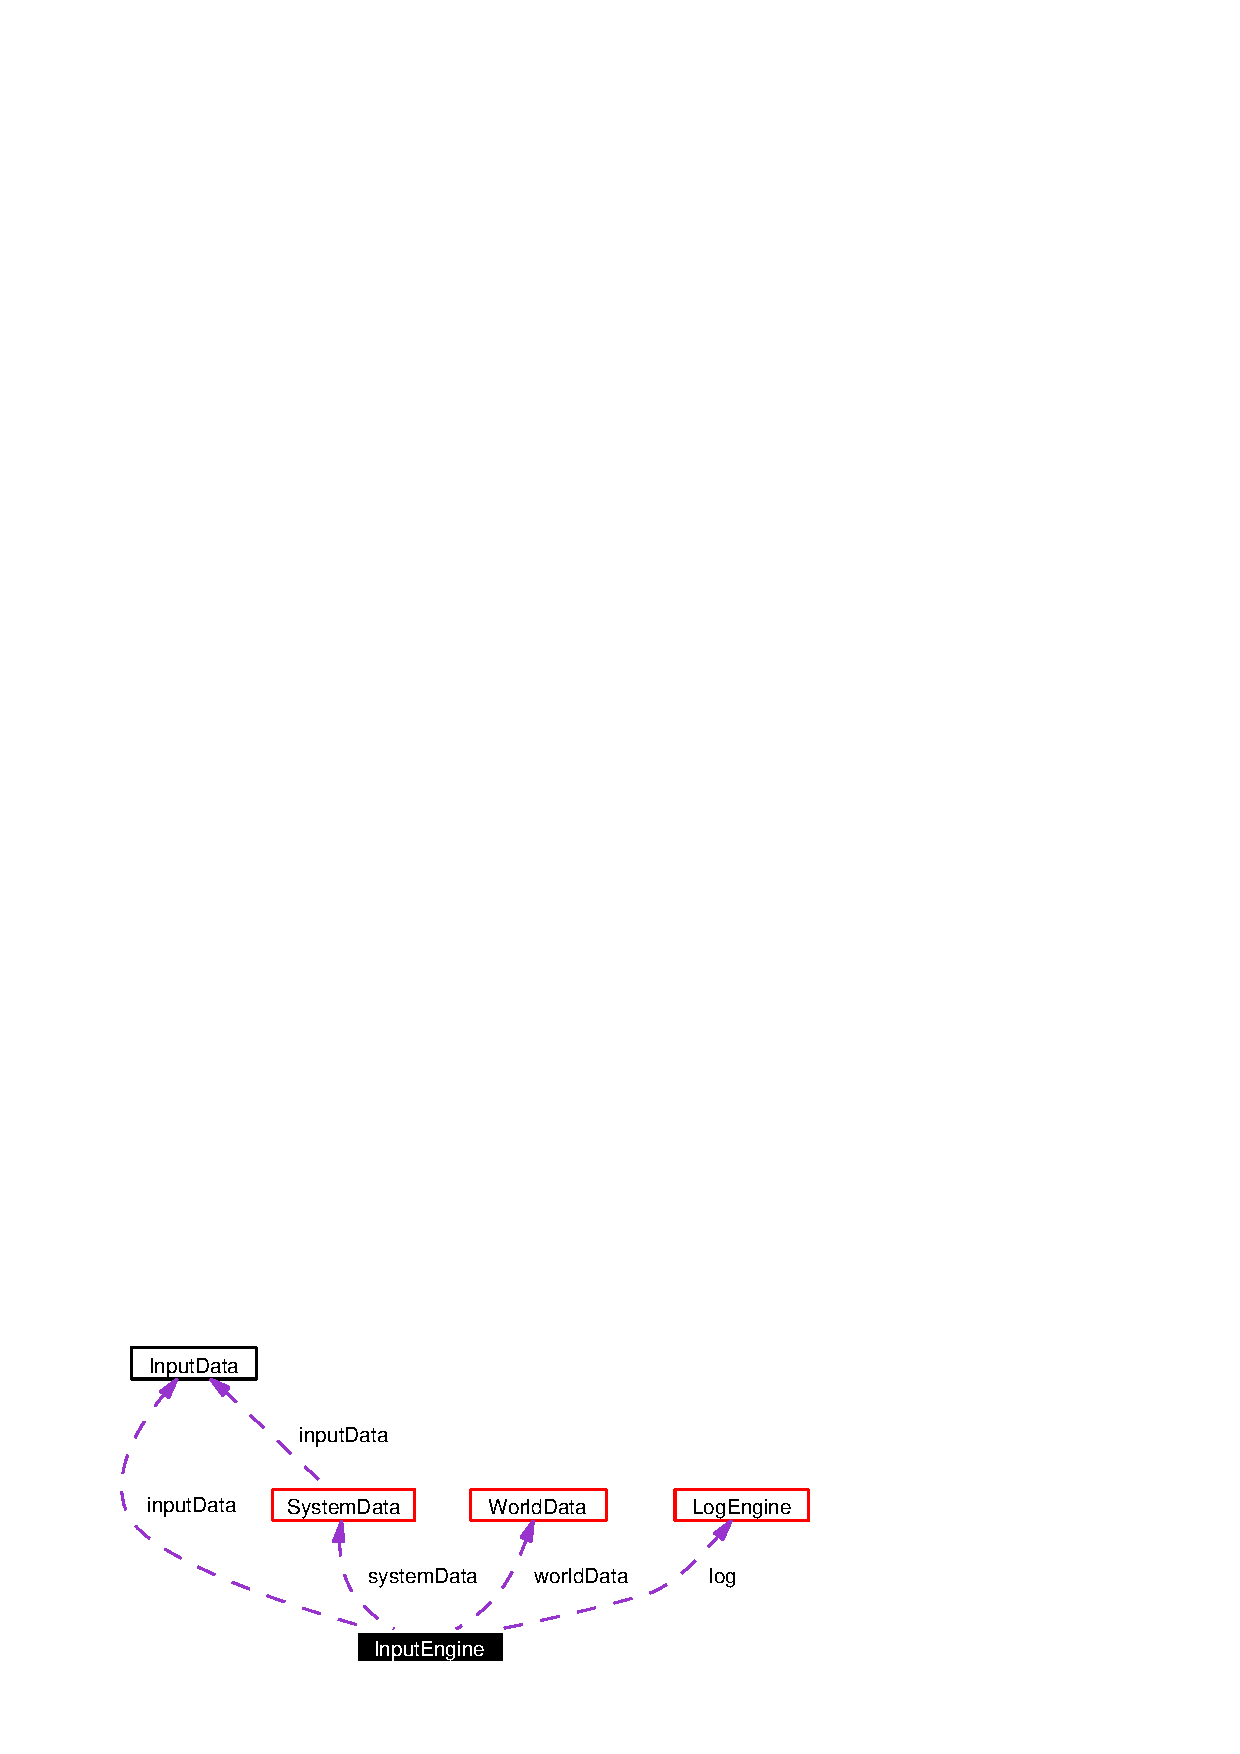
\includegraphics[width=194pt]{classInputEngine__coll__graph}
\end{center}
\end{figure}
\subsection*{Public Member Functions}
\begin{CompactItemize}
\item 
int {\bf start} ({\bf World\-Data} $\ast$wrl\-Data, {\bf System\-Data} $\ast$sys\-Data)
\item 
int {\bf step} (void)
\item 
void {\bf process\-Input} (SDLKey key\-Symbol)
\item 
int {\bf stop} (void)
\end{CompactItemize}
\subsection*{Private Attributes}
\begin{CompactItemize}
\item 
{\bf Log\-Engine} {\bf log}
\item 
{\bf Input\-Data} $\ast$ {\bf input\-Data}
\item 
{\bf System\-Data} $\ast$ {\bf system\-Data}
\item 
{\bf World\-Data} $\ast$ {\bf world\-Data}
\end{CompactItemize}


\subsection{Member Function Documentation}
\index{InputEngine@{Input\-Engine}!processInput@{processInput}}
\index{processInput@{processInput}!InputEngine@{Input\-Engine}}
\subsubsection{\setlength{\rightskip}{0pt plus 5cm}void Input\-Engine::process\-Input (SDLKey {\em key\-Symbol})}\label{classInputEngine_a2}


\index{InputEngine@{Input\-Engine}!start@{start}}
\index{start@{start}!InputEngine@{Input\-Engine}}
\subsubsection{\setlength{\rightskip}{0pt plus 5cm}int Input\-Engine::start ({\bf World\-Data} $\ast$ {\em wrl\-Data}, {\bf System\-Data} $\ast$ {\em sys\-Data})}\label{classInputEngine_a0}


\index{InputEngine@{Input\-Engine}!step@{step}}
\index{step@{step}!InputEngine@{Input\-Engine}}
\subsubsection{\setlength{\rightskip}{0pt plus 5cm}int Input\-Engine::step (void)}\label{classInputEngine_a1}


\index{InputEngine@{Input\-Engine}!stop@{stop}}
\index{stop@{stop}!InputEngine@{Input\-Engine}}
\subsubsection{\setlength{\rightskip}{0pt plus 5cm}int Input\-Engine::stop (void)}\label{classInputEngine_a3}




\subsection{Member Data Documentation}
\index{InputEngine@{Input\-Engine}!inputData@{inputData}}
\index{inputData@{inputData}!InputEngine@{Input\-Engine}}
\subsubsection{\setlength{\rightskip}{0pt plus 5cm}{\bf Input\-Data}$\ast$ {\bf Input\-Engine::input\-Data}\hspace{0.3cm}{\tt  [private]}}\label{classInputEngine_r1}


\index{InputEngine@{Input\-Engine}!log@{log}}
\index{log@{log}!InputEngine@{Input\-Engine}}
\subsubsection{\setlength{\rightskip}{0pt plus 5cm}{\bf Log\-Engine} {\bf Input\-Engine::log}\hspace{0.3cm}{\tt  [private]}}\label{classInputEngine_r0}


\index{InputEngine@{Input\-Engine}!systemData@{systemData}}
\index{systemData@{systemData}!InputEngine@{Input\-Engine}}
\subsubsection{\setlength{\rightskip}{0pt plus 5cm}{\bf System\-Data}$\ast$ {\bf Input\-Engine::system\-Data}\hspace{0.3cm}{\tt  [private]}}\label{classInputEngine_r2}


\index{InputEngine@{Input\-Engine}!worldData@{worldData}}
\index{worldData@{worldData}!InputEngine@{Input\-Engine}}
\subsubsection{\setlength{\rightskip}{0pt plus 5cm}{\bf World\-Data}$\ast$ {\bf Input\-Engine::world\-Data}\hspace{0.3cm}{\tt  [private]}}\label{classInputEngine_r3}




The documentation for this class was generated from the following files:\begin{CompactItemize}
\item 
src/input/{\bf input\-Engine.hpp}\item 
src/input/{\bf input\-Engine.cpp}\end{CompactItemize}
